\hypertarget{the-somatic-sensory-system}{%
\chapter{The Somatic Sensory System}\label{the-somatic-sensory-system}}

The somatic sensory system is a part of the sensory nervous system. The somatosensory system is a complex system of sensory neurons and neural pathways that responds to changes at the surface or inside the body. The axons (as afferent nerve fibers) of sensory neurons connect with, or respond to, various receptor cells. These sensory receptor cells are activated by different stimuli such as heat and nociception, giving a functional name to the responding sensory neuron, such as a thermoreceptor which carries information about temperature changes. Other types include mechanoreceptors, chemoreceptors, and nociceptors which send signals along a sensory nerve to the spinal cord where they may be processed by other sensory neurons and then relayed to the brain for further processing. Sensory receptors are found all over the body including the skin, epithelial tissues, muscles, bones and joints, internal organs, and the cardiovascular system.

Somatic senses are sometimes referred to as somesthetic senses, with the understanding that somesthesis includes the sense of touch and proprioception (sense of position and movement).

The mapping of the body surfaces in the brain is called somatotopy. In the cortex, it is also referred to as the cortical homunculus. This brain-surface (``cortical'') map is not immutable, however. Dramatic shifts can occur in response to stroke or injury.

\hypertarget{touch}{%
\section{Touch}\label{touch}}

In contrast, the other sense, touch, is a somatic sense which does not have a specialized organ but comes from all over the body, most noticeably the skin but also the internal organs (viscera). Touch includes mechanoreception (pressure, vibration and proprioception), pain (nociception) and heat (thermoception), and such information is carried in general somatic afferents and general visceral afferents.

Skin is the soft outer tissue covering of vertebrates with three main functions: protection, regulation, and sensation.



\begin{figure}

{\centering \includegraphics[width=0.7\linewidth]{./figures/somatosensory/Gray940} 

}

\caption{\href{https://commons.wikimedia.org/wiki/File:Gray940.png}{Diagramatic secion of hairless skin. Note tactile (Meissner) and Pacinian corpuscles.}}\label{fig:skindiagram}
\end{figure}

\hypertarget{cutaneous-mechanoreceptors}{%
\section{Cutaneous Mechanoreceptors}\label{cutaneous-mechanoreceptors}}

Cutaneous mechanoreceptors respond to mechanical stimuli that result from physical interaction, including pressure and vibration. They are located in the skin. They are all innervated by Aβ fibers, except the mechanorecepting free nerve endings, which are Aδ fibers. Cutaneous mechanoreceptors can be categorized by morphology, by what kind of sensation they perceive, and by the rate of adaptation. Furthermore, each has a different receptive field.



\begin{figure}

{\centering \includegraphics[width=0.7\linewidth]{./figures/somatosensory/mechano_sensitive_channel} 

}

\caption{A cartoon representation of the mechanosensitive Piezo1 channel in side and top view. \href{https://www.rcsb.org/structure/5Z10}{PDB 5Z10}, rendered with open source molecular visualization tool PyMol.}\label{fig:mechanosensitive}
\end{figure}

In the somatosensory system, receptive fields are regions of the skin or of internal organs. Some types of mechanoreceptors have large receptive fields, while others have smaller ones. Large receptive fields allow the cell to detect changes over a wider area, but lead to a less precise perception. Thus, the fingers, which require the ability to detect fine detail, have many, densely packed (up to 500 per cubic cm) mechanoreceptors with small receptive fields (around 10 square mm), while the back and legs, for example, have fewer receptors with large receptive fields.

Tactile-sense-related cortical neurons have receptive fields on the skin that can be modified by experience or by injury to sensory nerves resulting in changes in the field's size and position. In general these neurons have relatively large receptive fields (much larger than those of dorsal root ganglion cells). However, the neurons are able to discriminate fine detail due to patterns of excitation and inhibition relative to the field which leads to spatial resolution.

The term receptive field was first used by Sherrington (1906) to describe the area of skin from which a scratch reflex could be elicited in a dog. According to Alonso and Chen (2008) it was Hartline (1938) who applied the term to single neurons, in this case from the retina of a frog.

A sensory space can also map into a particular region on an animal's body. For example, it could be a hair in the cochlea or a piece of skin, retina, or tongue or other part of an animal's body.

This concept of receptive fields can be extended further up the nervous system; if many sensory receptors all form synapses with a single cell further up, they collectively form the receptive field of that cell. For example, the receptive field of a ganglion cell in the retina of the eye is composed of input from all of the photoreceptors which synapse with it, and a group of ganglion cells in turn forms the receptive field for a cell in the brain. This process is called convergence.

Tactile corpuscles or Meissner's corpuscles are a type of mechanoreceptor discovered by anatomist \href{https://en.wikipedia.org/wiki/Georg_Meissner}{Georg Meissner} (1829--1905) and \href{https://en.wikipedia.org/wiki/Rudolf_Wagner}{Rudolf Wagner}. They are a type of nerve ending in the skin that is responsible for sensitivity to light touch. In particular, they have their highest sensitivity (lowest threshold) when sensing vibrations between 10 and 50 hertz. They are rapidly adaptive receptors. They are most concentrated in thick hairless skin, especially at the finger pads.

Tactile corpuscles are encapsulated myelinated nerve endings, which consist of flattened supportive cells arranged as horizontal lamellae surrounded by a connective tissue capsule. The corpuscle is 30--140 μm in length and 40--60 μm in diameter. A single nerve fiber meanders between the lamellae and throughout the corpuscle.

Pacinian corpuscles (or lamellar corpuscles; discovered by Italian anatomist \href{https://en.wikipedia.org/wiki/Filippo_Pacini}{Filippo Pacini}) are one of the four major types of mechanoreceptor cell in glabrous (hairless) mammalian skin. They are nerve endings in the skin responsible for sensitivity to vibration and pressure. They respond only to sudden disturbances and are especially sensitive to vibration. The vibrational role may be used to detect surface texture, e.g., rough vs.~smooth. Pacinian corpuscles are also found in the pancreas, where they detect vibration and possibly very low frequency sounds.{[}dubious -- discuss{]} Pacinian corpuscles act as very rapidly adapting mechanoreceptors. Groups of corpuscles respond to pressure changes, e.g.~on grasping or releasing an object.

Pacinian corpuscles are larger and fewer in number than Meissner's corpuscle, Merkel cells and Ruffini's corpuscles.

The Pacinian corpuscle is approximately oval-cylindrical-shaped and 1 mm in length. The entire corpuscle is wrapped by a layer of connective tissue. Its capsule consists of 20 to 60 concentric lamellae (hence the alternative lamellar corpuscle) including fibroblasts and fibrous connective tissue (mainly Type IV and Type II collagen network), separated by gelatinous material, more than 92\% of which is water.

Pacinian corpuscles are rapidly adapting (phasic) receptors that detect gross pressure changes and vibrations in the skin. Any deformation in the corpuscle causes action potentials to be generated by opening pressure-sensitive sodium ion channels in the axon membrane. This allows sodium ions to influx, creating a receptor potential.

These corpuscles are especially susceptible to vibrations, which they can sense even centimeters away. Their optimal sensitivity is 250 Hz, and this is the frequency range generated upon fingertips by textures made of features smaller than 1 µm. Pacinian corpuscles cause action potentials when the skin is rapidly indented but not when the pressure is steady, due to the layers of connective tissue that cover the nerve ending. It is thought that they respond to high-velocity changes in joint position. They have also been implicated in detecting the location of touch sensations on handheld tools.

Pacinian corpuscles have a large receptive field on the skin's surface with an especially sensitive center.

Merkel cells, also known as Merkel-Ranvier cells or tactile epithelial cells, are oval-shaped mechanoreceptors essential for light touch sensation and found in the skin of vertebrates. They are abundant in highly sensitive skin like that of the fingertips in humans, and make synaptic contacts with somatosensory afferent nerve fibers. Although uncommon, these cells may become malignant and form a Merkel cell carcinoma---an aggressive and difficult to treat skin cancer.

Though it has been reported that Merkel cells are derived from neural crest cells, more recent experiments in mammals have indicated that they are in fact epithelial in origin.



\begin{figure}

{\centering 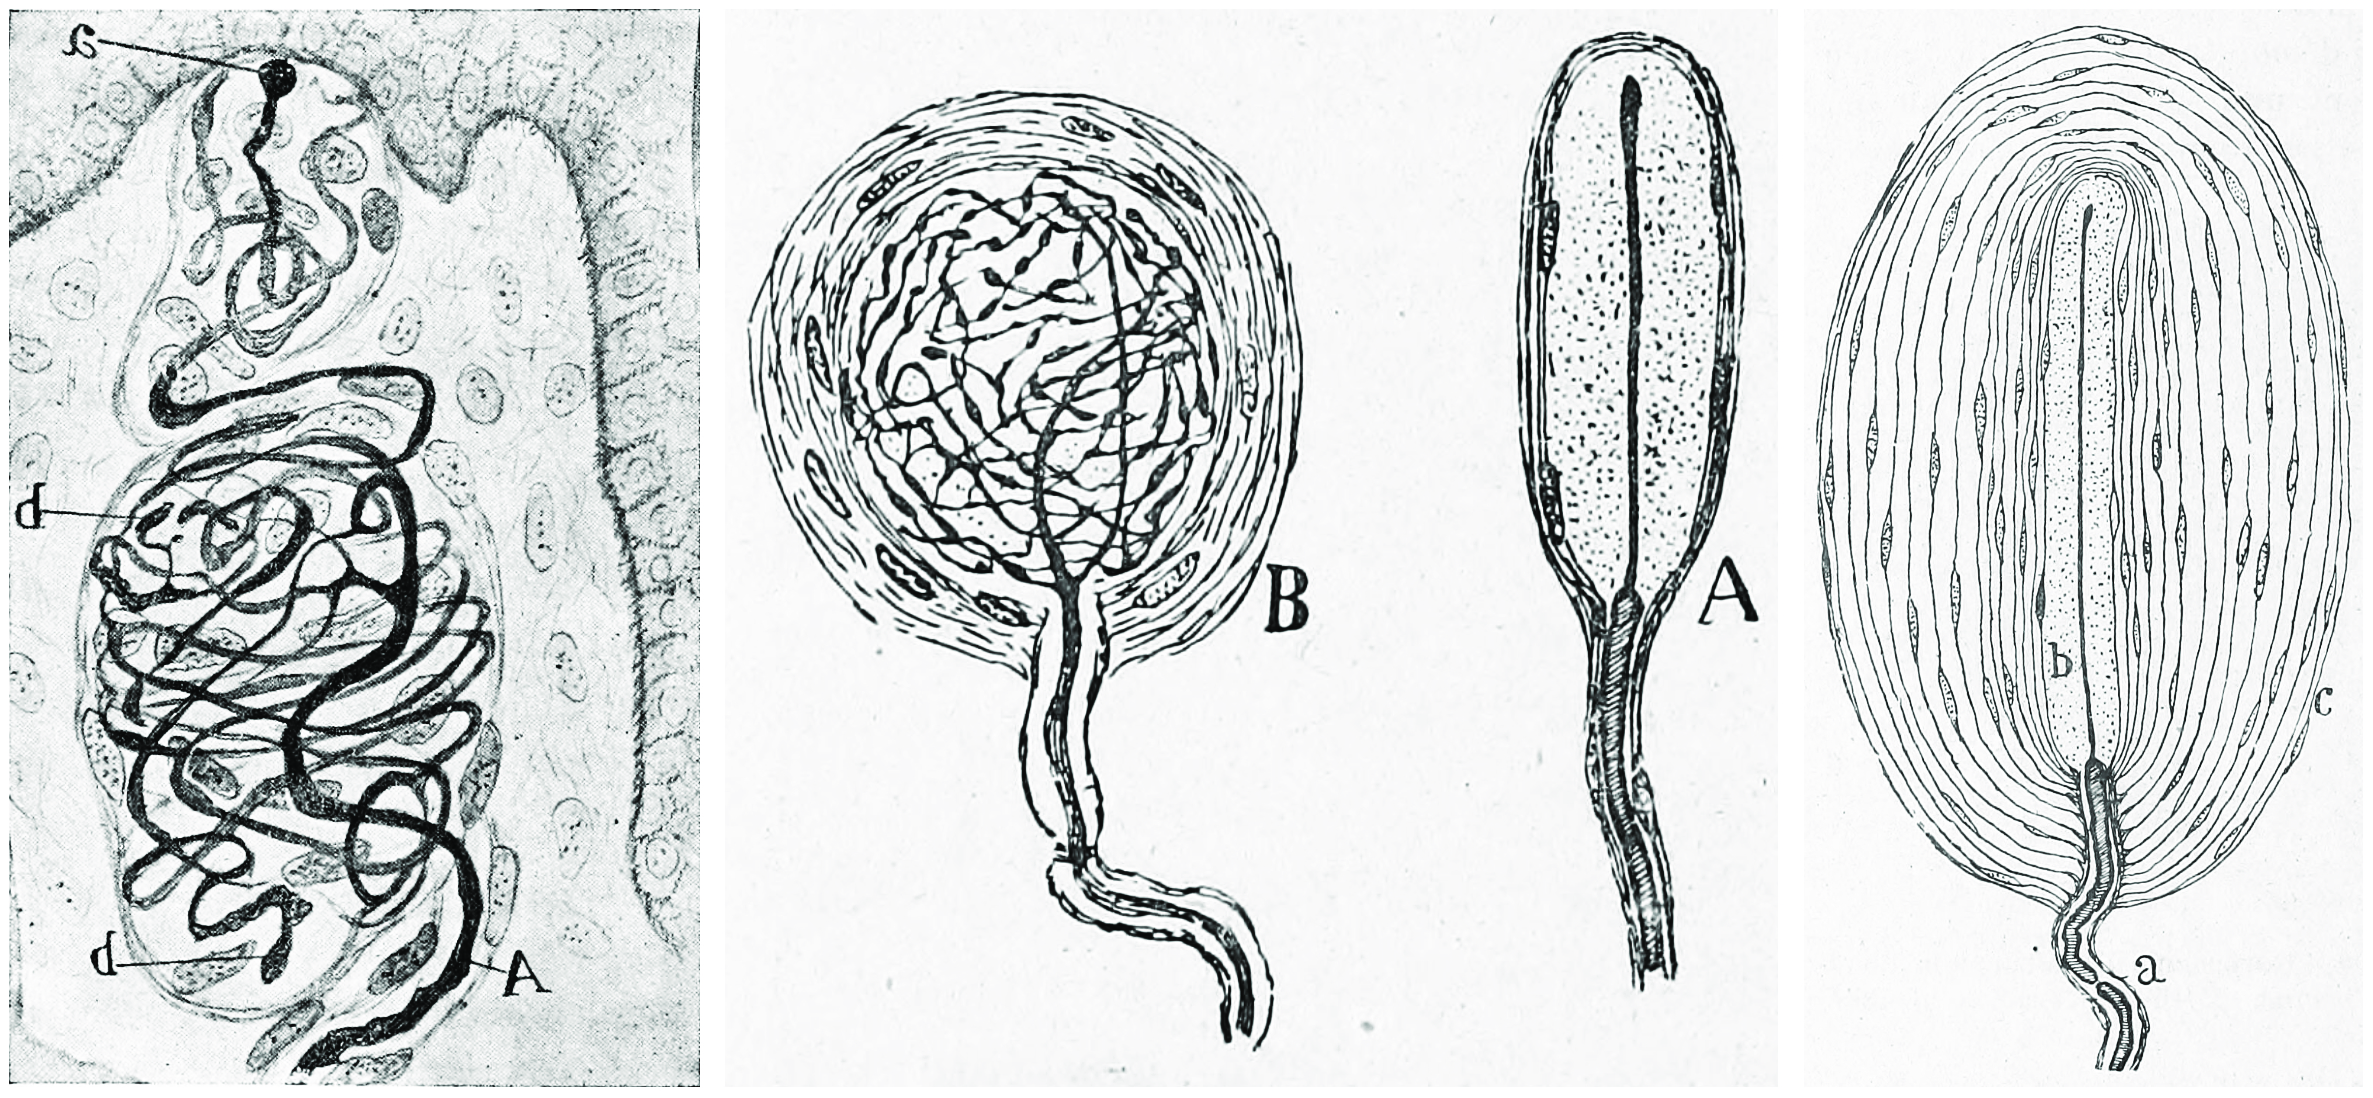
\includegraphics[width=0.7\linewidth]{./figures/somatosensory/TouchReceptors} 

}

\caption{\href{https://commons.wikimedia.org/wiki/File:Gray940.png}{Tactile corpuscles (from left to right): Meissner, Krause, Pacini}}\label{fig:tactilecorpuscle}
\end{figure}

Merkel cells are found in the skin and some parts of the mucosa of all vertebrates. In mammalian skin, they are clear cells found in the stratum basale (at the bottom of sweat duct ridges) of the epidermis approximately 10 μm in diameter. They also occur in epidermal invaginations of the plantar foot surface called rete ridges. Most often, they are associated with sensory nerve endings, when they are known as Merkel nerve endings (also called a Merkel cell-neurite complex). They are associated with slowly adapting (SA1) somatosensory nerve fibers. They react to low vibrations (5--15 Hz) and deep static touch such as shapes and edges. Due to a small receptive field (extremely detailed info) they are used in areas like fingertips the most; they are not covered (shelled) and thus respond to pressures over long periods.

The German anatomist \href{https://en.wikipedia.org/wiki/Friedrich_Sigmund_Merkel}{Friedrich Sigmund Merkel} referred to these cells as Tastzellen or ``touch cells'' but this proposed function has been controversial as it has been hard to prove. Though, genetic knockout mice have recently shown that Merkel cells are essential for the specialized coding by which afferent nerves resolve fine spatial details. Merkel cells are sometimes considered APUD cells (an older definition. More commonly classified as a part of dispersed neuroendocrine system) because they contain dense core granules, and thus may also have a neuroendocrine function.

The bulboid corpuscles (end-bulbs of Krause) are cutaneous receptors in the human body. The end-bulbs of Krause were named after the German anatomist \href{https://en.wikipedia.org/wiki/Wilhelm_Krause}{Wilhelm Krause} (1833--1910). End-bulbs are found in the conjunctiva of the eye (where they are spheroidal in shape in humans, but cylindrical in most other animals), in the mucous membrane of the lips and tongue, and in the epineurium of nerve trunks. They are also found in the penis and the clitoris and have received the name of genital corpuscles. The end-bulbs of Krause were thought to be thermoreceptors, sensing cold temperatures, but their function is unknown.

The Bulbous corpuscle or Ruffini ending or Ruffini corpuscle is a slowly adapting mechanoreceptor located in the cutaneous tissue between the dermal papillae and the hypodermis. It is named after Angelo Ruffini.

Ruffini corpuscles are enlarged dendritic endings with elongated capsules.

This spindle-shaped receptor is sensitive to skin stretch, and contributes to the kinesthetic sense of and control of finger position and movement. They are at the highest density around the fingernails where they act in monitoring slippage of objects along the surface of the skin, allowing modulation of grip on an object.

Ruffini corpuscles respond to sustained pressure and show very little adaptation.

Ruffinian endings are located in the deep layers of the skin, and register mechanical deformation within joints, more specifically angle change, with a specificity of up to 2.75 degrees, as well as continuous pressure states. They also act as thermoreceptors that respond for a long time, so in case of deep burn there will be pain, as these receptors will be burned off.

\hypertarget{nociception}{%
\section{Nociception}\label{nociception}}

\href{https://en.wikipedia.org/wiki/Nociception}{Nociception} (also nocioception or nociperception, from Latin nocere `to harm or hurt') is the sensory nervous system's response to certain harmful or potentially harmful stimuli. The term ``nociception'' was coined by \href{https://en.wikipedia.org/wiki/Charles_Scott_Sherrington}{Charles Scott Sherrington} to distinguish the physiological process (nervous activity) from pain (a subjective experience). In nociception, intense chemical (e.g., cayenne powder), mechanical (e.g., cutting, crushing), or thermal (heat and cold) stimulation of sensory nerve cells called nociceptors produces a signal that travels along a chain of nerve fibers via the spinal cord to the brain. Nociception triggers a variety of physiological and behavioral responses and usually results in a subjective experience of pain in sentient beings. Nociception can also cause generalized autonomic responses before or without reaching consciousness to cause pallor, sweating, tachycardia, hypertension, lightheadedness, nausea and fainting.

Potentially damaging mechanical, thermal, and chemical stimuli are detected by nerve endings called nociceptors, which are found in the skin, on internal surfaces such as the periosteum, joint surfaces, and in some internal organs. Some nociceptors are unspecialized free nerve endings that have their cell bodies outside the spinal column in the dorsal root ganglia. Nociceptors are categorized according to the axons which travel from the receptors to the spinal cord or brain.

Nociceptors have a certain threshold; that is, they require a minimum intensity of stimulation before they trigger a signal. Once this threshold is reached a signal is passed along the axon of the neuron into the spinal cord.

Nociceptive threshold testing deliberately applies a noxious stimulus to a human or animal subject in order to study pain. In animals, the technique is often used to study the efficacy of analgesic drugs and to establish dosing levels and period of effect. After establishing a baseline, the drug under test is given and the elevation in threshold recorded at specified time points. When the drug wears off, the threshold should return to the baseline (pre-treatment) value.

In some conditions, excitation of pain fibers becomes greater as the pain stimulus continues, leading to a condition called hyperalgesia.

Thermoception refers to stimuli of moderate temperatures 24--28 °C (75--82 °F), as anything beyond that range is considered pain and moderated by nociceptors. TRP and potassium channels {[}TRPM (1-8), TRPV (1-6), TRAAK, and TREK{]} each respond to different temperatures (among other stimuli) which create action potentials in nerves which join the mechano (touch) system in the posterolateral tract. Thermoception, like proprioception, is then covered by the somatosensory system.

TRP channels that detect noxious stimuli (mechanical, thermal, and chemical pain) relay that info to nociceptors that generate an action potential. Mechanical TRP channels react to depression of their cells (like touch), thermal TRP change shape in different temperatures, and chemical TRP act like taste buds, signalling if their receptors bond to certain elements/chemicals.



\begin{figure}

{\centering \includegraphics[width=0.7\linewidth]{./figures/somatosensory/TRPV1} 

}

\caption{A cartoon representation of the transient receptor potential cation channel subfamily V member 1 (TRPV1), also known as the capsaicin receptor and the vanilloid receptor 1 viewd from the side and the top. The function of TRPV1 is detection and regulation of body temperature. In addition, TRPV1 provides a sensation of scalding heat and pain (nociception). In primary afferent sensory neurons, it cooperates with TRPA1 (a chemical irritant receptor) to mediate the detection of noxious environmental stimuli. \href{https://www.rcsb.org/structure/5IS0}{PDB 5IS0}, rendered with open source molecular visualization tool PyMol.}\label{fig:TRPV1channel}
\end{figure}

\hypertarget{proprioception}{%
\section{Proprioception}\label{proprioception}}

Proprioception is the sense of self-movement and body position. It is sometimes described as the ``sixth sense''.

Proprioception is mediated by mechanically sensitive proprioceptor neurons distributed throughout an animal's body. Most vertebrates possess three basic types of proprioceptors: muscle spindles, which are embedded in skeletal muscle fibers, Golgi tendon organs, which lie at the interface of muscles and tendons, and joint receptors, which are low-threshold mechanoreceptors embedded in joint capsules. Many invertebrates, such as insects, also possess three basic proprioceptor types with analogous functional properties: chordotonal neurons, campaniform sensilla, and hair plates.

The initiation of proprioception is the activation of a proprioreceptor in the periphery. The proprioceptive sense is believed to be composed of information from sensory neurons located in the inner ear (motion and orientation) and in the stretch receptors located in the muscles and the joint-supporting ligaments (stance). There are specific nerve receptors for this form of perception termed ``proprioreceptors''.

An important role for proprioception is to allow an animal to stabilize itself against perturbations. For instance, for a person to walk or stand upright, they must continuously monitor their posture and adjust muscle activity as needed to provide balance. Similarly, when walking on unfamiliar terrain or even tripping, the person must adjust the output of their muscles quickly based on estimated limb position and velocity. Proprioceptor reflex circuits are thought to play an important role to allow fast and unconscious execution of these behaviors, To make control of these behaviors efficient, proprioceptors are also thought to regulate reciprocal inhibition in muscles, leading to agonist-antagonist muscle pairs.

When planning complex movements such as reaching or grooming, animals must consider the current position and velocity of their limb and use it to adjust dynamics to target a final position. If the animal's estimate of their limb's initial position is wrong, this can lead to a deficiency in the movement. Furthermore, proprioception is crucial in refining the movement if it deviates from the trajectory.

\hypertarget{muscle-spindles}{%
\section{Muscle Spindles}\label{muscle-spindles}}

Muscle spindles are stretch receptors within the body of a muscle that primarily detect changes in the length of the muscle. They convey length information to the central nervous system via afferent nerve fibers. This information can be processed by the brain as proprioception. The responses of muscle spindles to changes in length also play an important role in regulating the contraction of muscles, for example, by activating motor neurons via the stretch reflex to resist muscle stretch.



\begin{figure}

{\centering \includegraphics[width=0.7\linewidth]{./figures/somatosensory/CajalMuscleSpindle} 

}

\caption{Muscle spindle from the pectoral muscle of a frog. Bottom part of figure: B) extrafusal muscle fibers with efferent motor nerve; top part of figure: myelinated afferent nerve fiber. \href{https://wellcomelibrary.org/item/b2129592x\#?c=0\&m=0\&s=0\&cv=14\&z=0\%2C-3.48\%2C1\%2C8.6591}{Histologie du système nerveux de l'homme \& des vertébrés, Tome Premier} (1909) by Santiago Ramón y Cajal translated from Spanish by Dr.~L. Azoulay.}\label{fig:musclespindle}
\end{figure}

Muscle spindles are found within the belly of muscles, between extrafusal muscle fibers.{[}b{]} The specialised fibers that constitute the muscle spindle are known as intrafusal fibers (as they are present within the spindle), to distinguish themselves from the fibres of the muscle itself which are called extrafusal fibers. Muscle spindles have a capsule of connective tissue, and run parallel to the extrafusal muscle fibers.

\hypertarget{golgi-tendon-organ}{%
\section{Golgi Tendon Organ}\label{golgi-tendon-organ}}

The Golgi tendon organ (GTO) (also called Golgi organ, tendon organ, neurotendinous organ or neurotendinous spindle) is a proprioceptive sensory receptor organ that senses changes in muscle tension. It lies at the origins and insertion of skeletal muscle fibers into the tendons of skeletal muscle. It provides the sensory component of the Golgi tendon reflex.



\begin{figure}

{\centering \includegraphics[width=0.7\linewidth]{./figures/somatosensory/CajalGolgiTendon} 

}

\caption{Golgi tendon organ from an adult cat. a) Termninal arboriasation and c) fine ultimate brances of the afferent nerve; b) myelinated afferent nerve fiber; e) muscle fibers. \href{https://wellcomelibrary.org/item/b2129592x\#?c=0\&m=0\&s=0\&cv=14\&z=0\%2C-3.48\%2C1\%2C8.6591}{Histologie du système nerveux de l'homme \& des vertébrés, Tome Premier} (1909) by Santiago Ramón y Cajal translated from Spanish by Dr.~L. Azoulay.}\label{fig:tendonorgan}
\end{figure}

The body of the organ is made up of braided strands of collagen (intrafusal fasciculi) that are less compact than elsewhere in the tendon and are encapsulated. The capsule is connected in series with a group of muscle fibers (10-20 fibers) at one end, and merge into the tendon proper at the other. Each capsule is about 1 mm long, has a diameter of about 0.1 mm, and is perforated by one or more afferent type Ib sensory nerve fibers (Aɑ fiber), which are large (12-20 μm) myelinated axons that can conduct nerve impulses very rapidly. Inside the capsule, the afferent fibers lose their medullary sheaths, branch, intertwine with the collagen fibers, and terminate as flattened leaf-like endings between the collagen strands (see figure).

\hypertarget{the-somatosensory-pathways}{%
\section{The Somatosensory Pathways}\label{the-somatosensory-pathways}}

All afferent touch/vibration info ascends the spinal cord via the posterior (dorsal) column-medial lemniscus pathway via gracilis (T7 and below) or cuneatus (T6 and above). Cuneatus sends signals to the cochlear nucleus indirectly via spinal grey matter, this info is used in determining if a perceived sound is just villi noise/irritation. All fibers cross (left becomes right) in the medulla.

A somatosensory pathway will typically have three neurons: first-order, second-order, and third-order.

\begin{enumerate}
\def\labelenumi{\arabic{enumi}.}
\tightlist
\item
  The first-order neuron is a type of pseudounipolar neuron and always has its cell body in the dorsal root ganglion of the spinal nerve with a peripheral axon innervating touch mechanoreceptors and a central axon synapsing on the second-order neuron. If the somatosensory pathway is in parts of the head or neck not covered by the cervical nerves, the first-order neuron will be the trigeminal nerve ganglia or the ganglia of other sensory cranial nerves).
\item
  The second-order neuron has its cell body either in the spinal cord or in the brainstem. This neuron's ascending axons will cross (decussate) to the opposite side either in the spinal cord or in the brainstem.
\item
  In the case of touch and certain types of pain, the third-order neuron has its cell body in the ventral posterior nucleus of the thalamus and ends in the postcentral gyrus of the parietal lobe in the primary somatosensory cortex (or S1).
\end{enumerate}

Fine touch (or discriminative touch) is a sensory modality that allows a subject to sense and localize touch. The form of touch where localization is not possible is known as crude touch. The posterior column--medial lemniscus pathway is the pathway responsible for the sending of fine touch information to the cerebral cortex of the brain.

Crude touch (or non-discriminative touch) is a sensory modality that allows the subject to sense that something has touched them, without being able to localize where they were touched (contrasting ``fine touch''). Its fibres are carried in the spinothalamic tract, unlike the fine touch, which is carried in the dorsal column. As fine touch normally works in parallel to crude touch, a person will be able to localize touch until fibres carrying fine touch (Posterior column--medial lemniscus pathway) have been disrupted. Then the subject will feel the touch, but be unable to identify where they were touched.

In humans, temperature sensation from thermoreceptors enters the spinal cord along the axons of Lissauer's tract that synapse on second order neurons in grey matter of the dorsal horn. The axons of these second order neurons then decussate, joining the spinothalamic tract as they ascend to neurons in the ventral posterolateral nucleus of the thalamus.

\hypertarget{the-primary-somatosensory-cortex}{%
\section{The Primary Somatosensory Cortex}\label{the-primary-somatosensory-cortex}}

The primary somatosensory cortex is located in the postcentral gyrus, and is part of the somatosensory system.

At the primary somatosensory cortex, tactile representation is orderly arranged (in an inverted fashion) from the toe (at the top of the cerebral hemisphere) to mouth (at the bottom). However, some body parts may be mapped to partially overlapping regions of cortex. Each cerebral hemisphere of the primary somatosensory cortex only contains a tactile representation of the opposite (contralateral) side of the body. The amount of primary somatosensory cortex devoted to a body part is not proportional to the absolute size of the body surface, but, instead, to the relative density of cutaneous tactile receptors on that body part. The density of cutaneous tactile receptors on a body part is generally indicative of the degree of sensitivity of tactile stimulation experienced at said body part. For example, the human lips and hands have a larger representation than other body parts.

Brodmann areas 3, 1, and 2 make up the primary somatosensory cortex of the human brain (or S1). Brodmann area (BA) 3 is subdivided into areas 3a and 3b. Because Brodmann sliced the brain somewhat obliquely, he encountered area 1 first; however, from anterior to posterior, the Brodmann designations are 3, 1, and 2, respectively.

Areas 1 and 2 receive dense inputs from BA 3b. The projection from 3b to 1 primarily relays texture information; the projection to area 2 emphasizes size and shape. Lesions confined to these areas produce predictable dysfunction in texture, size, and shape discrimination.

Somatosensory cortex, like other neocortex, is layered. Like other sensory cortex (i.e., visual and auditory) the thalamic inputs project into layer IV, which in turn project into other layers. As in other sensory cortices, S1 neurons are grouped together with similar inputs and responses into vertical columns that extend across cortical layers.


